%%%%%%%%%%%%%%%%%%%%%%%%%%%%%%%%%%%%%%%%%%%%%%%%%%%%%%%%%%%%%%%%%%%%
%% chapter2.tex
%% NOVA thesis document file
%%
%% Chapter with the template manual
%%%%%%%%%%%%%%%%%%%%%%%%%%%%%%%%%%%%%%%%%%%%%%%%%%%%%%%%%%%%%%%%%%%%

\typeout{NT FILE chapter2.tex}%

\chapter{Background}
\label{cha:background}
\prependtographicspath{{Chapters/Figures/Covers/}}

% epigraph configuration
\epigraphfontsize{\small\itshape}
\setlength\epigraphwidth{12.5cm}
\setlength\epigraphrule{0pt}

This Chapter describes how to use the \gls{novathesis}\ template.  It is assumed that you have a working \index{installation} of \LaTeX, either local (in your own computer) or remote (in \Overleaf), and that you were able to generate a PDF for the default configuration of the template: a PhD thesis for \gls{FCT}.
This Chapter aims at exemplifying how to do common stuff with \LaTeX. We also show some stuff which is not that common! ;)

Please, use these examples as a starting point, but you should always consider using the \emph{Big Oracle} (aka, \href{http://www.google.com}{Google}, your best friend) to search for additional information or al-ternative ways for achieving similar results.

\section{Replication} % (fold)
\label{sec:replication}
Replication is one of the cornerstones in the design of reliable distributed systems. It is a widely used technique to provide high availability, low latency and the ability to tolerate individual node losses (fault-tolerance). A replicated system is one in which multiple devices work together to replicate the behavior of the same system as if only a single device was responsible for the entirety of it.

There are several replication models and techniques one can choose when designing a replicated database system. Each approach to the system design can provide different properties to it. 

\subsection{Total and Partial Replication}
\label{sec:total_and_partial_replication}
When thinking about data location and availability, one can reason about the total and partial replication models. 

With total replication, every instance of the database has a complete copy of it’s state, meaning that every storage node contains all data available in the system. With this approach one can achieve high data availability, since data is available in every database instance, faster query execution and improved load balancing, since queries can be executed in any replica, especially when the system’s clients are scattered throughout the world, by having multiple instances of the data closer to the clients. On the other hand, since total replication requires that all replicas have their data synchronized at all times, it might introduce the problem of data consistency and slower update process.

In contrast, in the partial replication model, each replica only holds a subset of the database~\cite{partial-replication}. This can be an interesting approach when storage space is a concern because updates are propagated only towards the affected sites. However, certain sites are not able to execute certain types of transactions, which can affect the ability to load balance.

\subsubsection{Active and Passive Replication}
\label{sec:active_and_passive_replication}
The previous concepts, are mainly focused on addressing where data is being stored. However, it is also necessary to consider how data is replicated and how updates are propagated among the different replicas. The active and passive replication models provide two different methods of approaching this issue.

Active replication is a method in which client operations are forwarded to all replicas in a coordinated order, relying on a protocol to decide the order of execution of such operations. Afterwards, each replica executes the operations independently, reaching a result state identical among all replicas. With this approach, to guarantee that replicas state after executing all operations is identical, client operations are required to be deterministic~\cite{replication-state-of-the-art}.

When using passive replication, all client requests are sent to a primary node, which executes the requests and sends update messages, containing the state of the master after executing the request, to the secondary nodes in the same order as the order of the operations executed by the master replica. Unlike active replication, client operations are not required to be deterministic due to the fact that only the master node receives and executes requests. On the other hand, this approach can consume a lot of bandwidth when the result state is large. Also, the primary node might fail and, thus, this method is required to have a replica recovery and master election protocol~\cite{principles-of-eventual-consistency}.
% section document_structure (end)

\section{Consistency}
\label{sec:consistency}

A concerning aspect of replication is data consistency. It is required that replica’s state is consistent among all of them. Replica’s state being consistent means that if a client executes an operation, the result state of all replicas is identical, independently of which replica receives the client’s request. This can become an even harder challenge when multiple clients execute multiple operations in different replicas, especially if some of the operations are write operations. In that case, it is necessary to have a mechanism in place that assures that replicas always converge to the same state.

\subsection{Consistency Models}
\label{sec:consistency_models}
In distributed systems, a consistency model refers to the guarantees provided by the system about the order in which operations appear to occur to clients. It determines how data is accessed and updated across multiple nodes, and how these updates are made available to clients ~\cite{consistency-models}. There are several consistency models, each with its advantages and disadvantages, and can be categorized in two categories: data-centric, client-centric~\cite{consistency-models}.

When discussing consistency, read and write are the available operations to perform over a shared data item. When a process performs a read operation, it expects the return value to be the result of the last write operation performed on the given data item. However, it is not possible to have a global clock to synchronize operations and decide which write was performed last. Therefore, we need to provide alternatives that lead to a range of consistency models~\cite{distributed-systems-principles-paradigms}.

\subsection{Data-centric consistency models}
\label{sec:data_centric_consistency_models}
In the perspective of the data store, shared data is required to be stored consistently in all replicas. In order to achieve such requirement, it is necessary to establish protocols able to guarantee that data is up to date at all times in all replicas. Hence, data-centric models focus on the internal synchronization processes and the communication between replicas~\cite{towards-comprehensive-measurement-guarantees}.

\subsubsection{Strong Consistency Models}
\label{sec:strong_consistency_models}
A system provides strong consistency if, at all times, data is consistent among all replicas. This means that after receiving and executing client requests, all replicas should converge to a single consistent state, by executing the same request before replying to the client. With this type of consistency model, clients can send their requests to any node because they will always get the exact same response to a request, unless faults occurred in the system or in nodes. The downside of this kind of consistency models is that the synchronization requirements might be too demanding, which can negatively impact response latency because clients only get a response after the synchronization process has terminated.

\subsubsection{Linearizability}
One of the strongest consistency models is \textbf{\textit{Linearizability}}, in which, each operation has an associated point in time, called linearization point, which is the moment in time when the operation appears to take effect atomically, without the interference of other concurrent operations. Under linearizability, it is guaranteed that the systems behaves as if all operations ocurred in a sequential manner~\cite{linearizability-geeks}.

\subsubsection{Causal Consistency}
\label{sec:causal-consistency}
In the causal consistency model, operations have a causal relationship between them, i.e. if an operation A is dependent on the output of an operation B, then operation B must be executed before operation A. For example, if operation B reads a resource and operation A updates the value of the resource based on the value read by B, then A must be executed after B because A depends on B. With this model, it is guaranteed that a client does not read two related write operations in a wrong order and in case the client has read the latest value, then it does not read the stale value~\cite{consistency-models}.

\subsubsection{Weak Consistency}
\label{sec:weak_consistency}
A weak consistency model is one that provides the lowest possible guarantees on the ordering of operations. In simpler terms, weak consistency can be seen as an approach where replicas might by chance become consistent~\cite{consistency-in-distributed-systems}.

\subsection{Client-centric consistency models}
\label{sec:client_centric_consistency_models}
Client-centric consistency insures that while a client has access to a resource, it will never see an inconsistent state of the resource. However, if multiple clients have access to the same resource simultaneously, then consistency is not guaranteed~\cite{consistency-models}.

\subsubsection{Eventual Consistency}
\label{sec:eventual_consistency}

Eventual consistency guarantees that when a write operation is performed over a data store, that operation’s result will eventually be reflected in all replicas where the updated data item is stored(tese luis chula). 

This model is a form of weak consistency, thus it isn’t required to synchronize replicas when clients send requests allowing for reduced latency. After a period of time, if no faults occur in the system or no write operations where performed, then eventually all replicas will converge to a single consistent state. However, since updates are performed asynchronously, if other clients read the data item from other replicas, it is not guaranteed that the operation will return the most recent write.

\subsubsection{Monotonic Reads}
\label{sec:monotonic_reads}

Monotonic reads ensure that when a client reads a version \textit{n} of a data item, future read operations on the same replica will always return a version of the data item equal or newer than \textit{n}~\cite{consistency-in-distributed-systems}. From an application perspective data visibility might not be instantaneous but versions become visible in chronological order. 

\subsubsection{Monotonic Writes}
\label{sec:monotonic_writes}

It is important that write operations are propagated in the correct order to all copies of a data store. In a monotonic write consistent store, a write operation by a process on a data item k is completed before successive write operation on \textit{k} by the same process. Therefore, a write operation on a copy of k is performed only if that copy has been brought up to date by means of any preceding write operation, which may have taken place on other copies of \textit{k}. In case old writes have not finished, the new write must wait for old ones to finish~\cite{distributed-systems-principles-paradigms}.

\subsubsection{Read Your Writes}
\label{sec:read_your_writes}

A data store provides read-your-writes consistency, if the effect of a write operation by a process on data item \textit{k} will always be seen by a successive read operation on \textit{k} by the same process(distributed systems principles and paradigms). This condition guarantees that a write operation is always completed before a successive read operation by the same process, no matter where that read operation takes place. 
% subsection with_a_remote_cloud_based_service (end)

\subsubsection{Writes Follow Reads}
\label{sec:writes_follow_reads}

Write follows reads consistency guarantees that any successive write operation by a process on a data item \textit{k} will be performed on a copy of \textit{k} that is up to date with the value most recently~\cite{distributed-systems-principles-paradigms}.

A data store provides write follows reads consistency, if a write operation by a process on a data item \textit{k} following a previous read operation on \textit{k} by the same process is guaranteed to take place on the same or a more recent value of \textit{k} that was read

\section{Publish/Subscribe Systems}
\label{sec:pub_sub}

A \gls{pubsub} system is one in which clients communicate asynchronously between them by exchanging notifications, relying on a notification service, also known as \textit{broker} interposed between them~\cite{large-content-based-pubsub-systems}. In this systems there are two type of clients, producers and consumers, more often called publishers ans subscribers, respectively.

Producers publish events and consumers subscribe to events by issuing subscriptions. Consumers can have multiple active subscriptions and after issuing one, the event service is responsible for delivering all future notifications when publishers publish an event, subscribed by the subscriber, until the subscription gets canceled. This allows consumers to express their interest in an event or pattern of events. Figure ~\ref{fig:pub_sub_architecture} shows the architecture of \gls{pubsub} systems with a single broker. 

This kind of system is a great choice for applications focused on information dissemination, such as newsletters.

\begin{figure}[htbp]
    \centering
    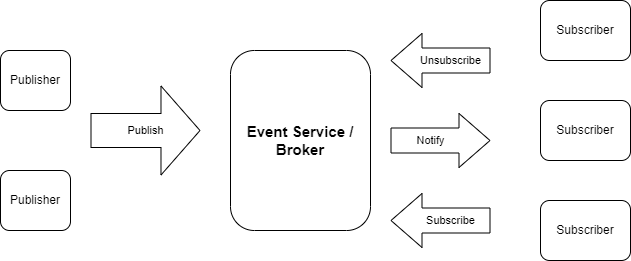
\includegraphics[width=0.8\linewidth]{Chapters/Figures/pubsub_architecture.drawio.png}
    \caption{Publish/Subscribe architecture}
    \label{fig:pub_sub_architecture}
\end{figure}

\subsection{Event Service}
\label{sec:event_service}

The \gls{pubsub} system model relies on an event notification service responsible for storing publications, managing subscriptions and efficiently delivering notifications to subscribers~\cite{faces-of-pub-sub}. It acts as a middle-man between publishers and subscribers allowing these to be decoupled from each other.

The decoupling provided can be decomposed into three dimension~\cite{faces-of-pub-sub}:

\begin{itemize}
    \item \textbf{Space decoupling}: publishers and subscribers are not required to know each other by relying on the event service to receive publications from publishers and delivering notifications to subscribers;
    \item \textbf{Time decoupling}: publishers and subscribers do not need to actively participate in the interaction at the same time. Publishers can publish events while subscribers are disconnected and subscribers can be notified of events while the original publisher of the event is disconnected;
    \item \textbf{Synchronization decoupling}: publishers do not get blocked while publishing events and subscribers get notified asynchronously of an event while performing other concurrent tasks.
\end{itemize}

\subsection{Subscription schemes}
\label{sec:subscription_model}

Subscribers are often more interested in a specific set of events rather than all events. Thus, subscriptions had to be adapted to allow subscribers to specify the set of events they were most interested, which lead to the creation of several subscription schemes. The most widely used subscription schemes are the following~\cite{faces-of-pub-sub}:

\begin{itemize}
    \item \textbf{Topic-based subscription}: participants publish events and subscribe to individual topics, identified by keywords;
    \item \textbf{Content-based subscription}: consumers subscribe to events by specifying filters to event's content. Filters are rules that must be met by the content of a publication in order to get notified by the event service.
    \item \textbf{Type-based subscription}: extends topic-based subscription by introducing the notion of types.
\end{itemize}

\subsubsection{Topic-Based Publish/Subscribe}
\label{sec:topic-based-poubsub}

This thesis will mainly focus on a topic-based \gls{pubsub} system, therefore, this section goes into more detail about this type of system.

In topic-based systems, messages are associated with topics and are routed selectively to destinations with matching interests. Topics are associated with channels, which are queues of messages maintained by brokers, and it’s name is used to create the channel. After creation, every channel is uniquely identified by it’s name, also used as an argument for the publish() and subscribe() functions. Clients can subscribe to multiple topics and will receive future messages published to those topics~\cite{pubsub-systems-book}.

As stated in~\cite{faces-of-pub-sub}, the concept of topics is similar to the concept of groups in the context of group communication. Also, subscriptions can be seen as joining a group and publishing a message as broadcasting that message to the members of that group.

\subsection{Reliable Publish/Subscribe Systems}
\label{sec:reliable_pub_sub_systems}

When dealing with distributed systems, it is generally required to add components to systems due to higher service demands and geographical positioning of clients. However, the more components a system is composed of, the more complex it becomes and the probability of components failing also increases.

In general, in distributed systems, \textbf{faults} can be defined as the deviation of a component from it's correct behavior. In order to develop a reliable system, it is important to make assumptions about how a process might fail. Therefore, it is of extreme importance to define a fault model.

\begin{table}[H]
\rowcolors{1}{}{GhostWhite}
\begin{xltabular}{\textwidth}{cX}
  \caption{Process fault models based on~\cite{fault-tolerance-distributed-systems}.}
  \label{tab:fault_models}\\
  \toprule
  \rowcolor{Gainsboro}
  Type & Description\\
  \midrule
  Crash Model & When a process fails it stops sending messages\\
  \hline
  Omission Model & After failing, a process omits the trasmission or reception of any number of messages\\
  \hline
  Fail-Stop Model & Upon failure, the process "notifies" all other processes of its own failure and stops sending messages\\
  \hline
  Byzantine Model & A process might deviate from its behavior in an arbitrary way\\
  \bottomrule
\end{xltabular}
\end{table}

Table~\ref{tab:fault_models} displays some of the most common process failures that can be observed in systems. However, a system also requires the presence of a network, which enables communication between processes but is also prone to failures.

% \begin{table}[H]
%   \rowcolors{1}{}{GhostWhite}
%   \begin{xltabular}{\textwidth}{cX}
%     \caption{Network failures}
%     \label{tab:network_failures}\\
%     \toprule
%     \rowcolor{Gainsboro}
%     Failure & Description\\
%     \midrule
%     Link Failure & Links between processes become unavailable\\
%     \hline
%     Device Failure & Ne
%     \hline
%     Message Loss & Messages sent from a process to another might get lost for non-deterministic reasons\\
%     \bottomrule
%   \end{xltabular}
%   \end{table}

Detecting failures can seem to be a trivial task, however when dealing with very wide systems, it might present itself as a bigger challenge. Therefore, it is important to design robust systems and algorithms able to guarantee the correct behavior of correctly operating processes, in the presence of such failures. 

In the context of distributed \gls{pubsub} systems, it is often necessary to provide strong guarantees about the reliable delivery of information. This is mainly due to publishers and subscribers being decoupled as mentioned in section \ref{sec:pub_sub}. Systems can rely, for example, on overlay networks of distributed brokers or group communication and reliable application-layer multicast, such as Scribe~\cite{scribe}, to propagate messages between brokers and from publishers to subscribers~\cite{faces-of-pub-sub}.

Moreover, we should also take into account that brokers might eventually fail and, therefore, system's need to implement mechanisms to detect such failures and recover from them.

In ~\cite{tutorial-on-reliability-in-pubsub}, the authors highlight some techniques and strategies that have been adopted by current implementations:

\begin{itemize}
  \item \textbf{Planning}: estimate the reliability level of several paths from a source to a destination, and pick the one that exposes the highest reliability. This mainly aims at avoiding faults as much as possile;
  \item \textbf{Reconfiguration}: adopt topological reconfiguration to recover connectivity in the forwarding tree after a node or link crashes. It aims at maintaining a consistent connectivity for the system;
  \item \textbf{Retrasmissions}: publishers store produced events so that subscribers can request retransmissions when losses are somehow detected;
  \item \textbf{Epidemic Algorithms}: each process exchanges at a random time its history of the received notifications with a randomly-chosen set of processes among the ones constituting the system. Subsequently, inconsistencies, i.e., message drops are detected by comparison and corrected through retransmissions;
  \item \textbf{Forward Error Correction}: forward redudant data instead of using retransmissions. This way the receiver can reconstruct te original event even if some notifications have been dropped during delivery;
  \item \textbf{Broker Replication}: replicates the brokers in the notification service. The state of a broker is replicated to its neighbors so in case of a broker failure, it can be easily substituted without losing subscription consistency;
  \item \textbf{Path Redundancy}: establishes redundant pathes among the nodes of the system. Notifications are sent through multiple paths, and only the first-received replica of the message is delivered to the   
\end{itemize}

The following sections go over some approaches taken by researchers to address the reliability problem of \gls{pubsub} systems.

\subsubsection{Epidemic Algorithms for Reliable Content-Based Publish-Subscribe: An Evaluation}
\label{sec:reliable_gossip}

In the papers ~\cite{epidemic-algs-for-pubsub} and ~\cite{intro-epidemic-algs-for-pubsub}, the authors approach reliability by relying in gossip (or epidemic) algorithms to improve reliability in content-based \gls{pubsub} systems and propose three algorithms based on different gossip strategies.

Unlike topic-based \gls{pubsub} where topic subscriptions define a group of receivers and messages within a topic can be assigned a sequence number to easily detect losses, patterns in content-based \gls{pubsub} do not have the same effect. This is mainly linked to the fact that events can match multiple patterns resulting in routing being performed independently and messages not getting assigned a sequence number. The authors identify the previous problems as the main challenges that have to be addressed when applying reliability to content-based \gls{pubsub}

In gossip algorithms, when a node wants to propagate a message to every node, instead of broadcasting the message, it picks a subset of the nodes, from the set of nodes in the system, to send the message to and when each node receives the message, each repeats the process. There are two main types of gossip: \textit{push} and \textit{pull}. In \textit{push} gossip, each node gossips periodically, to disseminate its view of the system to other processes, while in \textit{pull} gossip, a node requests the trasmission of information from other nodes to compensate local losses.

The first proposed algorithm, uses a strategy based on \textit{push} gossip. At each gossip round, the gossiper randomly picks a pattern \textit{p} from its subsciption table, constructs a digest, a pair containing the source identifier and a sequence number associated top the source, of the identifiers of all the cached events matching \textit{p}, builds a gossip message containing the digest, labels it with \textit{p} and propagates the message. Afterwards, when a dispatcher receives a message labelled with \textit{p}, it checks if it is subscribed to this pattern and if the indentifiers contained in the digest correspond to events already received by it. The identifiers of missed events are included in a request message sent to the gossiper, which replies by sending the corresponding events.

The second and third algorithms use a strategy based on \textit{pull} gossip. The former is a \textit{subscriber-based} algorithm in which, when a dispatcher detects a lost event it inserts the corresponding information in a buffer \textit{Lost}. In the next gossip round, it chooses a pattern \textit{p} among the ones associated with local subscriptions, selects the events in \textit{Lost} related with it, and inserts the corresponding information in a digest attached to a new gossip message. The message is then labelled with \textit{p} and routed similarly to the \textit{push} solution. Afterwards, when a dispatcher receives the message, it checks its  cache against the events requested by the gossiper and, if any are found, sends them back to it. The last solution is a \textit{publisher-based} algorithm. It requires that event sources also cache their published events and that the address of each dispatcher on the path towards a subscriber is appended to the message. It behaves similarly to the previous algorithm, but instead routes gossip messages towards publishers instead of publishers. The messages are distinguished based on the event source rather than the pattern, and augmented with the information required to route back to the publisher.

\subsubsection{Fault-Tolerant Reliable Delivery of Messages in Distributed Publish/Subscribe Systems}
\label{sec:fault_tolerant_reliable_delivery}

In ~\cite{repository-nodes}, the authors present a gossip-based approach to reliable delivery of messages over a reliable-topic, that relies on a special kind of node, which manages a set of reliable-topics, called \textit{repository} node. The \textit{repository} facilitates reliable delivery from multiple publishers to multiple subscribers. Managing a reliable-topic involves two key components:
\begin{enumerate}
  \item The \textit{repository} should facilitate the registration and de-registration of authorized entities for reliable communications; and
  \item The \textit{repository} must support error-corrections, retransmissions and recovery from failures.
\end{enumerate}

Reliable delivery of messages also involves two key aspects:
\begin{enumerate}
  \item The \textit{repository} needs to ensure that messages published by the publisher, over a reliable-topic are stored exactly-once, without gaps and in order at the repository managing this reliable-topic; and
  \item The \textit{repository} has to compute the intended destinations and ensure the reliable delivery of the stored message to the computed destinations.
\end{enumerate}

The authors found that the use of a \textit{repository} node, to manage reliable-topics, would result in clients having to wait for the \textit{repository} to recover in case of failures, therefore becoming a single point of failure. To address this issue, each reliable-topic is managed by a set of \textit{repositories}, called a \textit{repository bundle}. Every \textit{repository} inside a \textit{repository bundle}, must manage the same reliable-topics. This solution provides redundancy, high-availability and more fault-tolerance.

\subsubsection{Reliable and Highly Available Distributed Publish/Subscribe Service}
\label{sec:reliable_and_highly_available_distributed_pubsub}

In ~\cite{reliable-highly-available-pub-sub}, the authors present a system that uses a topology management and subscription propagation scheme that enables brokers to compute new forwarding paths when failures of nearby neighbors occur.

The systems relies on a tree-based overlay, in which brokers maintain a partial view of this tree which includes all brokers within distance \textit{f+1}, where \textit{f} is the maximum number of concurrent broker failures that the algorithm tolerates. Such information is stored locally by each broker in a data structure called the  topology map.

Brokers also maintain a subscription table containing entries for subscriptions inserted into the system. Subscriptions contain a \textit{from} field that points to another broker located \textit{f+1} hops closer to the subscriber. In the event of failure of one or more neighbors, the broker uses this information and its topology map to reconnect the network topology, and forward publications over new paths towards matching subscribers.

Finally, the algorithm contains a recovery procedure used by failed brokers to re-enter the system. This procedure aims at restoring a broker's routing information according to the current state of the network and is divided in three phases: \textit{synchronization}, \textit{message forwarding} and \textit{termination of recovery}.  

\subsubsection{MinAvg-kTCO}
\label{sec:minavg_tco}

In the paper ~\cite{minavg-k-tco}, the authors propose the \textit{MivAvg-kTCO} problem parameterized by \textit{k} to use the minimum number of edges to create a \textit{k-topic-connected overlay ({kTCO})} for \gls{pubsub} systems.

A \textit{topic connected overlay (TCO)} is a per-topic connected graph of nodes subscribed to the topic, where exists a path between each pair nodes without being directly connected. Using \textit{TCOs} guarantees that nodes not interested in that topic, do not contribute to disseminate information on that topic. The downside of \textit{TCOs} is that connectivity is not guaranteed even if a single node fails. To address this issue, the authors introduce \textit{k-topic-connected-overlay (kTCO)} which guarantee connectivity if fewer than \textit{k} nodes fail simultaneously for the same topic.

The authors conclude the paper by presenting two algorithms that solve the \textit{MivAvg-kTCO} problem: GM\textit{2} to build \textit{2}TCOs and Harary-Per-Topic (HPT) to build \textit{k}TCOs where \textit{k} is greater than 2.

\subsubsection{P2S}
\label{sec:p2s}

P2S~\cite{p2s}, is a topic-based and crash-tolerant \textit{Paxos}-based \gls{pubsub} middleware based on Goxos, a \textit{Paxos}-based State Machine Replication framework. Paxos is a fault-tolerant consensus protocol in which a set of replicas tries to reach agreement on a value. With this protocol, replicas can reach agreement when at least \textit{f+1} replicas are able to communicate, where \textit{f} is the number of failures the system can tolerate.

This system leverages Paxos as a way to achieve total message ordering, while providing a mechanism to tolerate broker failures. For that purpose, P2S relies on a set of \textit{2f+1} brokers between publishers and subscribers. With this design, P2S is able to provide fault-tolerance through replication while providing total ordering through Paxos.

In this system, client messages are handled by the Goxos framework. When clients send messages, Goxos treats them as Paxos requests, orders and delivers them to the broker application layer, which forwards the messages to the subscribers according to the message topic.

%\newpage

\begin{sidewaystable}
%\begin{table}
\small
\rowcolors{1}{}{GhostWhite}
\begin{xltabular}{\textwidth}{cccccccX}
  \caption{Solution properties.}
  \label{tab:solution_properties}\\
  \toprule
  \rowcolor{Gainsboro}
  System & Topology & Delivery & Ordering & Fault-tolerance & Strategy & Details & Requirements\\
  \midrule
  ~\ref{sec:reliable_and_highly_available_distributed_pubsub} & Tree & Exactly-once & FIFO & \checkmark & Redundant Edges & Partial view & Each broker maintains in its partial view all replicas within $\delta$+1 distance, where $\delta$ is the number of faults to tolerate\\
  P2S~\cite{p2s} & Star & X & Total & \checkmark & Paxos & Replicates broker & 2f+1 replicas, where f is the number of faults to tolerate\\
\end{xltabular}%
%\end{table}
\end{sidewaystable}

%\begin{tabularx}{\textwidth}{ 
%  | >{\raggedright\arraybackslash}X 
%  | >{\centering\arraybackslash}X 
%  | >{\raggedleft\arraybackslash}X | }
%  \caption{Properties of presented solutions}
%  \label{tab:solution_properties}\\
%  \hline
%  System& Topology& Delivery Guarantees& Ordering Guarantees& Fault-tolerance& How& Details\\
%  \hline
%  P2S& star& X& T& Total& Paxos& Replcating the broker& To tolerate failures of f+1 replicas requires 2f+1 nodes\\
%\end{tabularx}

\section{Example glossary, acronyms, and symbols}
%
% \todo[inline]{A a note in a line by itself.}
%
This is the first occurrence of an abbreviation: \gls{abbrev}. And now the second occurrence of the same abbreviation: \gls{abbrev}. And a new acronym with capital letter: \Gls{xpt} and reused \gls{xpt}.  Let's also use a few other acronyms such as \gls{aaa}, \gls{aab}, \gls{aba}, \gls{bbb} and \gls{xpt}.
In geometry, the area enclosed by a circle of radius \gls{r} is $\pi r^2$. Here the Greek letter \gls{pi} is equal to the ratio of the circumference of any circle to its diameter.
Lets add ``\gls{computer}'' to the glossary! Be carefull with mathematical symbols in acronyms, please see the definition of \gls{mu}.

% Reference to Potassium \gls{chem:potassio} and Sodium \gls{chem:sodio} as well.

%
% Please note that
% \begin{center}
%   \textbf{\large this package and template are not official for FCT/NOVA}.
% \end{center}



% \printbibliography[heading=subbibliography, segment=\therefsegment, title={\bibname\ for chapter~\thechapter}]


\endinput

%!TEX root = ../template.tex
%%%%%%%%%%%%%%%%%%%%%%%%%%%%%%%%%%%%%%%%%%%%%%%%%%%%%%%%%%%%%%%%%%%%
%% chapter2.tex
%% NOVA thesis document file
%%
%% Chapter with the template manual
%%%%%%%%%%%%%%%%%%%%%%%%%%%%%%%%%%%%%%%%%%%%%%%%%%%%%%%%%%%%%%%%%%%%

\typeout{NT FILE chapter2.tex}%

\chapter{NOVAthesis Template \emph{User's Manual}}
\label{cha:users_manual}

\glsresetall

\begin{center}
  \fbox{\LARGE
    This manual is outdated and must be revised!}
\end{center}

Referência ao Potássio é \gls{chem:potassio} e Sódio também \gls{chem:sodio}.

\section{Introduction}
\label{sec:introduction}

This chapter describes how to use the \gls{novathesis}\ Template and the \gls{novathesisclass} file.  I will assume you have a working installation of \LaTeX, wither local (in your own computer) or remote (in Overleaf), and that it compiled successfully the default configuration (PhD for \gls{FCT}).


\section{Folder Structure}
\label{sec:folder_structure}

The \gls{novathesis} template is organized into many files and folders. At the main level it includes the following files and folders:

\noindent
\bgroup
\rowcolors{1}{GhostWhite}{}
\begin{xltabular}{\linewidth}{>{\ttfamily}l>{\itshape}l>{\upshape}X}
novathesis.cls     & file    &
The main class file. It will include additional files from \texttt{NOVAthesisFiles} folder and its sub-folders.
\\
template.tex      & file    &
The main template file. You need to \emph{compile} this file with one of pdf\LaTeX, \XeLaTeX, or \LuaLaTeX\ to obtain the \texttt{template.pdf} file.
\\
bibliography.bib  & file    &
An example of a bibliography file. You may have has many as you want. \\
template.pdf      & file    &
A possible result of applying pdf\LaTeX\ to the \texttt{template.tex} file. The template supports multiple types of documents (e.g., MSc dissertation, PhD thesis, …) and multiple Schools (e.g., FCT-NOVA, FCSH-NOVA, IST-UL, FC-UL, …) and each will produce different results.
\\
Chapters          & folder  & Examples of thesis chapters. Replace them with your own chapters.
\\
Examples          & folder  & Some more examples of the use of the template for different document types and Schools.
\\
Scripts           & folder  & Some (possibly useful) scripts for Unix-based systems (Linux, Mac OSx). If you are a windows user, ignore this folder (you may safely delete it if you want).
\\
NOVAthesisFiles   & folder  &
Additional files for the \gls{novathesisclass}\ file.  Unless you know what you are doing, avoid messing up with the files and folders inside this folder (except for deleting the unused Schools, see below).
\\
\end{xltabular}
\egroup

The \texttt{NOVAthesisFiles} folder contains additional files and folders that complement the main \gls{novathesisclass}\ file.  These are:

\noindent
\bgroup
\rowcolors{1}{GhostWhite}{}
\begin{tabularx}{\linewidth}{>{\ttfamily}l>{\itshape}l>{\upshape}X}
README.txt      & file    &
A file that should be read!  :)
\\
fix-babel.tex   & file    &
Simple fixes to the \texttt{babel} package.
\\
lang-text.ldf   & file    &
Translations of important strings used in the template.  Currently fully supported are Portuguese and English, but French is on the way.  If you add translations for your own language, please be so kind and send them to me. Thank you!
\\
options.tex     & file    &
Processing of \gls{novathesisclass}\ options.  \emph{Don't mess with this!}
\\
packages.tex    & file    &
Additional packages to be loaded into the \gls{novathesis}\ template. \emph{You should not mess with this!}
\\
spine.tex       & file    &
This file is loaded only if the option \texttt{spine=full} or \texttt{spine=trim}, and includes the typesetting of the book spine.
\\
ChapStyles      & folder  &
Contains a lot of files, one for each chapter style.  If you really know what you are doing, you may add your own chapter style here.
\\
FontStyles      & folder  &
Contains a few files, one for each set of fonts (main text font, chapter font, section font, subsection font, etc).  If you really know what you are doing, you may add your own set here.
\\
Schools         & folder  &
Configuration files for each school.  This folder is organized into subfolders, one for each university.  \emph{You may safely delete all the subfolders except the one for your University.}  Then open the subfolder of your University and \emph{you may safely delete all the subfolders except the one for your School/Faculty}.
\\
\end{tabularx}
\egroup

As stated above, the \texttt{Schools} folder contains per-university folders and per-school (faculty) subfolders.  Currently these are the available folders:

\noindent
\bgroup
\rowcolors{1}{GhostWhite}{}
\begin{tabularx}{\linewidth}{>{\ttfamily}r@{~/~}>{\ttfamily}l>{\itshape}l>{\upshape}X}
ul     & ist    & folder  &
The folder for the \href{http://www.tecnico.ulisboa.pt}{\emph{Instituto Superior Técnico}} of the \emph{University of Lisbon}.
\\
nova    & fcsh   & folder  &
The folder for the \href{http:www.fcsh.unl.pt}{\emph{Faculty of Human and Social Sciences}}  of the \emph{NOVA University of Lisbon}.
\\
nova    & fct    & folder  &
The folder for the \href{http:www.fct.unl.pt}{\emph{Faculty of Sciences and Technology}} of the \emph{NOVA University of Lisbon}.
\\
nova    & novaims    & folder  &
The folder for the \href{http:www.novaims.unl.pt}{\emph{Information and Management School}} of the \emph{NOVA University of Lisbon}.
\\
\end{tabularx}
\egroup

% section folder_structure (end)

% ===================
% = Package options =
% ===================
\section{\glsfmtshort{novathesisclass}\ Class Options}
\label{sec:package_options}

The \gls{novathesisclass}\ can be customized with the options listed below.

\newcommand{\classoption}[3]{\textbf{#1=OPT}\qquad #2\\\qquad\emph{#3}\\}

\noindent
\begin{ctabular}{@{}p{\linewidth}@{}}
  \toprule
%----------------------------------------------------------------------
  \classoption{doctype}%
    {phd(*), phdplan, phdprop, msc, mscplan, bsc}%
    {The type of the document: PhD Thesis (---~Default~---), PhD Plan, PhD Proposal, MSc Dissertation, MSc Plan, BSc Report}
    \midrule
%----------------------------------------------------------------------
  \classoption{school}%
    {nova/fct(*), nova/fcsh, nova/ims, ul/ist, ul/fc}%
    {The name of the school. This option changes the typesetting of the cover and some School specific formating, like margins, fonts, paragraph spacing and indentation, etc…}
    \midrule
%----------------------------------------------------------------------
  \classoption{lang}%
    {en(*), pt}%
    {The main language for the document.  Currently only Portuguese and English are supported.  Other languages are expected to be support in forthcoming versions.}
    \midrule
%----------------------------------------------------------------------
  \classoption{fontstyle}%
    {bookman, charter, fourier, kpfonts(*), mathpazo1, mathpazo2, newcent}%
    {The font set to be used in the document.  Please note that a font set include definitions for the main text, headings, maths, etc.}
    \midrule
%----------------------------------------------------------------------
%----------------------------------------------------------------------
  \classoption{chapstyle}%
    {bianchi, bluebox, brotherton, dash, default, elegant(*), ell, ger, hansen, ist, jenor, lyhne, madsen, pedersen, veelo, vz14, vz34, vz43}%
    {The chapter style, i.e., the look of the chapter beginning.}
    \midrule
%----------------------------------------------------------------------
  \classoption{converlang}%
    {en, pt(*)}%
    {The language to be used when typesetting the cover page.}
    \midrule
%----------------------------------------------------------------------
  \classoption{otherlistsat}%
    {front(*), back}%
    {Where to put the other lists besides the table of contents. The default is (\texttt{front}) before the main text.  But some scientific areas prefer them at the end of the document (\texttt{back}), just before the Appendixes.}
    \midrule
%----------------------------------------------------------------------
  \classoption{statement}%
    {true, false(*)}%
    {Include or don't include the contents of the “\texttt{statement}” file. The default is for this file to be ignored (if it exists).}
    \midrule
%----------------------------------------------------------------------
  \classoption{linkscolor}%
    {darkblue(*), black}%
    {The color for all the hyperlinks in the PDF file.  The “\texttt{media=paper}” option (see below) will override this option to “\texttt{black}”}
    \midrule
%----------------------------------------------------------------------
  \classoption{spine}%
    {true, false(*)}%
    {Generate the book spine and the last page in the PDF.}
    \midrule
%----------------------------------------------------------------------
  \classoption{biblatex}%
    {OPT=\{list of options for \texttt{biblatex}\}}%
    {Customize \texttt{biblatex}, the bibliography management system used in this class. Probably you will want to change the value of the \texttt{biblatex} “\texttt{style}” option. For other customizations of \texttt{biblatex} check its manual.}
    \midrule
%----------------------------------------------------------------------
  \classoption{memoir}%
    {OPT=\{list of options for \texttt{memoir}\}}%
    {Customize the base class \texttt{memoir}. The \texttt{memoir} manual should be the first document to be consulted when looking for “\textbf{how can I do this?}” You may what to change the base font size from 11pt to a smaller (10pt) or larger (12pt) size.  Also, remember to change the “\texttt{draft}” to final when your document is finished.}
    \midrule
%----------------------------------------------------------------------
  \classoption{media}%
    {screen(*), paper}%
    {Behavior to be customized in the school options/configuration. Expected definitions for screen are: left and right margins are equal and use colored links. Expected definitions for paper are: left and right margins are different and use black links.}
    \bottomrule
\end{ctabular}

\section{Additional considerations about the class options}
\label{sec:additional_considerations}

In this section we will provide some additional considerations about some of the customizations available as class options.

\subsection{The main language}
\label{sub:the_main_language}

The choice of the main language with the option “\texttt{lang=OPT}” affects:

\begin{itemize}
  \item \textbf{The order of the summaries.} First is printed the abstract in the main language and then in the foreign language. This means that if your main language for the document in English, you will see first the “abstract” (in English) and then the “resumo” (in Portuguese). If you switch the main language for the document for Portuguese, it will also automatically switch the order of the summaries to “resumo” and then “abstract”.
  \item \textbf{The names for document sectioning.} E.g., ``Chapter'' vs.\ ``Capítulo'', ``Table of Contents'' vs.\ ``Índice'', ``Figure'' vs.\ ``Figura'', etc.
  \item \textbf{The type of documents in the bibliography.} E.g., ``Technical Report'' vs.\ ``Relatório Técnico'', ``PhD Thesis'' vs.\ ``Tese de Doutoramento'', etc.
\end{itemize}

No mater which language you chose, you will always have the appropriate hyphenation rules according to the language at that point. You always get Portuguese hyphenation rules in the ``Resumo'', English hyphenation rules in the ``Abstract'', and then the main language hyphenation rules for the rest of the document.

% subsection the_main_language (end).

% section additional_consideration (end)


\subsection{Class of Text}
\label{sub:class_of_text}

You must choose the class of text for the document. The available options are:

\begin{enumerate}
  \item \textbf{bsc} --- BSc graduation report.
  \item \textbf{*mscplan} --- Preparation of MSc dissertation. This is a preliminary report graduate students at DI-FCT-NOVA must prepare to conclude the first semester of the two-semesters MSc work. The files specified by \verb!\ntdedicatoryfile! and \verb!\acknowledgmentsfile! are ignored, even if present, for this class of document.
  \item \textbf{msc} --- MSc dissertation.
  \item \textbf{phdprop} ---  Proposal for a PhD work. The files specified by \verb!\ntdedicatoryfile! and \verb!\acknowledgmentsfile! are ignored, even if present, for this class of document.
  \item \textbf{prepphd} ---  Preparation of a PhD thesis. This is a preliminary report PhD students at DI-FCT-NOVA must prepare before the end of the third semester of PhD work. The files specified by \verb!\ntdedicatoryfile! and \verb!\acknowledgmentsfile! are ignored, even if present, for this class of document.
  \item \textbf{phd} --- PhD dissertation.
\end{enumerate}
% subsection class_of_text (end)

% ============
% = Printing =
% ============
\subsection{Printing}
\label{sub:printing}

You must choose how your document will be printed. The available options are:
\begin{enumerate}
  \item \textbf{oneside} --- Single side page printing.
  \item \textbf{*twoside} --- Double sided page printing.
\end{enumerate}
% subsection printing (end)

% =============
% = Font Size =
% =============
\subsection{Font Size}
\label{ssec:font_size}

You must select the encoding for your text. The available options are:
\begin{enumerate}
  \item \textbf{11pt} --- Eleven (11) points font size.
  \item \textbf{*12pt} --- Twelve (12) points font size. You should really stick to 12pt\ldots
\end{enumerate}
% subsection font_size (end)

% =================
% = Text encoding =
% =================
\subsection{Text Encoding}
\label{ssec:text_encoding}

You must choose the font size for your document. The available options are:
\begin{enumerate}
  \item \textbf{latin1} --- Use Latin-1 (\href{http://en.wikipedia.org/wiki/ISO/IEC_8859-1}{ISO 8859-1}) encoding.  Most probably you should use this option if you use Windows;
  \item \textbf{utf8} --- Use \href{http://en.wikipedia.org/wiki/UTF-8}{UTF8} encoding.    Most probably you should use this option if you are not using Windows.
\end{enumerate}
% subsection font_size (end)

% ============
% = Examples =
% ============
\subsection{Examples}
\label{ssec:examples}

Let's have a look at a couple of examples:

\begin{itemize}
  \item Preparation of PhD thesis, in portuguese, with 11pt size and to be printed single sided (I wonder why one would do this!)\\
  \verb!\documentclass[prepphd,pt,11pt,oneside,latin1]{thesisdifct-nova}!
  \item MSc dissertation, in English, with 12pt size and to be printed double sided\\
  \verb!\documentclass[msc,en,12pt,twoside,utf8]{thesisdifct-nova}!
\end{itemize}
% subsection examples (end)

\section{How to Write Using \LaTeX}
\label{sec:how_to_write_using_latex}

Please have a look at Chapter~\ref{cha:a_short_latex_tutorial_with_examples}, where you may find many examples of \LaTeX constructs, such as Sectioning, inserting Figures and Tables, writing Equations, Theorems and algorithms, exhibit code listings, etc.

% section how_to_write_using_latex (end)



\section{Example glossary, acronyms, and symbols}
%
% \todo[inline]{A a note in a line by itself.}
%
This is the first occurrence of an abbreviation: \gls{abbrev}. And now the second occurrence of the same abbreviation: \gls{abbrev}. And a new acronym with capital letter: \Gls{xpt} and reused \gls{xpt}.  Let's also use a few other acronyms such as \gls{aaa}, \gls{aab}, \gls{aba}, \gls{bbb} and \gls{xpt}.
In geometry, the area enclosed by a circle of radius \gls{r} is $\pi r^2$. Here the Greek letter \gls{pi} is equal to the ratio of the circumference of any circle to its diameter.
Lets add ``\gls{computer}'' to the glossary! Be carefull with mathematical symbols in acronyms, please see the definition of \gls{mu}.
%
% Please note that
% \begin{center}
%   \textbf{\large this package and template are not official for FCT/NOVA}.
% \end{center}



% \printbibliography[heading=subbibliography, segment=\therefsegment, title={\bibname\ for chapter~\thechapter}]
